\chapter{Podstawy teoretyczne eksperymentu LHCb}

Ten rozdział pokrótce opisuje teoretyczne podstawy stojące za Fizyką Wysokich Energii (ang. \textbf{H}igh \textbf{E}nergy \textbf{P}hysics ).Na samym początku omówiona zostaje fundamentalna zasada fizyki. Następnie opisane zostają 

\section{Symetrie w fizyce}
Jeżeli chce się rozmawiać na temat fizyki zawsze powinno się zacząć od tematu symetrii. Jedną z najbardziej fundamentalnych zasad w fizyce jest ta, łącząca prawa zachowania z symetriami natury. Twierdzenie Noether pokazuje, że jeśli układ fizyczny jest niezmienniczy \footnote{w znaczeniu Lagranżjan opisujący ten układ} względem ciągłej transformacji, oznacza istnienie zachowanie pewnej wielkości. Niezmienniczość praw fizycznych względem translacji czasowej jest odpowiedzialne za istnienie zasady zachowania energii. Zasada zachowania pędu, natomiast pochodzi od niezmienniczości względem przesunięć w przestrzeni. Natomiast zasada zachowania pędu jest zachowana gdy prawa fizyki są identyczne zastosowaniu obrotów w przestrzeni. 

Poza, wyżej wymienionymi symetriami ciągłymi istnieją jeszcze symetrie dyskretne. Które, w przeciwieństwie do tych wcześniej opisanych mogą być łamane w pewnych fizycznych oddziaływaniach. Dla fizyki cząstek elementarnych istotnymi symetriami są:

\begin{itemize}
\item \textbf{C}- sprzężenie ładunkowe (ang. charge conjugation) zmienia znak wszystkich addytywnych numerów kwantowych. W specyficznym odniesieniu do rozpadów sub-atomowych cząstek, sprzężenie ładunkowe oznacza zamianę każdej cząstki na sprzężoną z nią antycząstkę.
\item \textbf{P}- parzystość (ang. parity) jest to operacja odwrócenia jednej z trzech przestrzennych osi.
\item \textbf{T} odwrócenie czasu (ang. time reversal) zmienia kierunek ruchu przez odbicie w czasie osi. 
\end{itemize}

Według obecnej wiedzy, każda z tych symetrii jest zachowana w oddziaływaniach silnych i elektromagnetycznych. Natomiast, co bardziej interesujące, słabe siły łamią symetrie \textbf{C} oraz \textbf{P}. Jednakże, kombinacja tych symetrii \textbf{CPT} jest dokładną symetrią w każdej lokalnej Lorentz'owskiej teorii pola.

\section{Symetrie a początek Wszechświata}
W przybliżeniu po okresie $10^{-6}s$ do Wielkiego Wybuchu została uformowana plazma gluonowo-kwarkowa w której to wolne kwarki oraz gluony podróżowały z relatywistycznymi prędkościami. Pary cząstka-antycząstka były stale tworzone oraz anihilowane, tworząc fotony, równomiernie poruszające się przez kosmos. Po tym procesie, do dzisiaj pozostają widzialne pamiątki nazywane Mikrofalowym promieniowaniem tła (ang. \textbf{C}osmic \textbf{M}icrowave \textbf{B}ackground). Na podstawie badań tego promieniowania oszacowano wiek Wszechświata na $13.75 \pm 0.11$ miliarda lat.

Niedługo, po tym jak CMB zostało wytworzone jedna liczb kwantowych \textit{liczba barionowa} została złamana, powodując, że więcej cząstek było produkowanych niż antycząstek. Ten proces nazywany \textit{bariogenezą} oznacza, że dzisiejszy wszechświat jest zbudowany z materii.

W 1967 Sacharow  wyjaśnił, że powodem dla którego we Wszechświecie brak jest antymaterii wymaga spełnienia trzech warunków:
\begin{enumerate}
\item Niezachowania liczby barionowej. 
\item Ochładzanie Wszechświata zachodziło w warunkach niebędących w równowadze termodynamicznej. 
\item Zachodzenie procesu łamania symetrii kombinowanej \textbf{CP} 
\end{enumerate}

\section{Symetria kombinowana \textbf{CP}}
Symetria kombinowana \textbf{CP}, będąca jak wcześniej wspomniano jednym z warunków Sacharowa do tego, aby istniał wszechświat, była poddana obserwacji już wcześniej. Powodem tego było odkryciem istnienia tylko lewoskrętnych\footnote{Skrętność oznacza rzut wektora spinu na kierunek ruchu cząstki} neutrin i prawoskrętnych antyneutrin. Wynikiem zastosowania operatora \textbf{CP}\footnote{Operatory \textbf{C} oraz \textbf{P} komutują ze sobą nawzajem} na neutrino lewoskrętne jest antyneutrino prawoskrętne. Stąd sądzono, że ta symetria jest zachowana przez oddziaływania słabe, obrazowo działania tych operatorów zostały zaprezentowane na rysunku \ref{fig:CP}.


 \begin{figure}[ht]
 \centering
 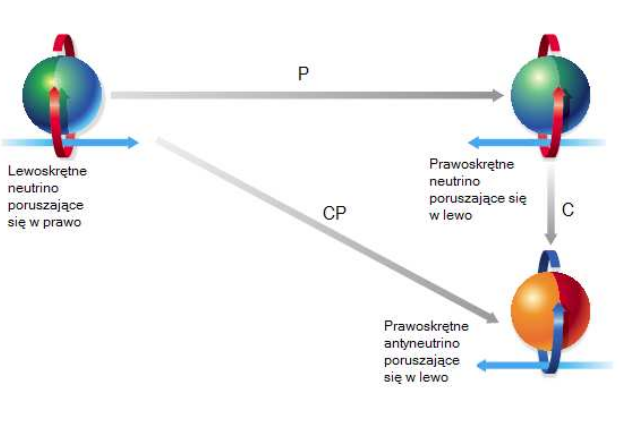
\includegraphics[scale=0.7]{rozdzial1/CP.png}
 % Beetle_block.jpeg: 848x489 pixel, 96dpi, 22.44x12.94 cm, bb=0 0 636 367
 \caption{Działanie operatorów C, P i CP na neutrino}
 \label{fig:CP}
\end{figure}


 Tak było do roku 1964, kiedy to w rozpad neutralnych kaonów pokazał, że ta symetria jednak jest łamana (więcej informacji ref ). Pierwszym dowodem na łamanie  \textbf{CP} poza układem kaonów, był zaobserwowany w 2001 roku przez kolaborację eksperymentu Belle. Badali oni układ neutralnych mezonów B\footnote{Mezon B to hadron składający się z kwarka b oraz lżejszy antykwark } . Odkrycie zapoczątkowało nową erę badań procesów łamiących symetrię  \textbf{CP}. Lekkie mezony B (neutralne $B_u$ oraz naładowane $B_d$ były poddawane precyzyjnym pomiarom przez fabryki-B: Belle(ref) oraz BaBar(ref). LHCb jest eksperymentem drugiej generacji. Właściwości eksperymentu, które będą omówione w następnym rozdziale, pozwalają na poszukiwania łamania \textbf{CP}  w sektorze mezonów $B_{s}$ oraz zjawisk Nowej Fizyki.
 \begin{figure}[ht]
 \centering
 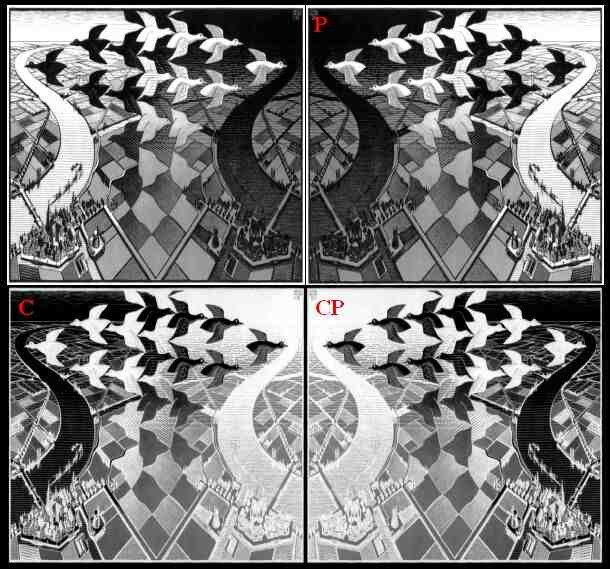
\includegraphics[scale=0.7]{rozdzial1/CPV.jpg}
 % Beetle_block.jpeg: 848x489 pixel, 96dpi, 22.44x12.94 cm, bb=0 0 636 367
 \caption{Artystyczne wizualizacja łamania symetrii \textbf{CP}. Sprzężenie ładunkowe zostało zaprezentowane jako zamiana kolorów, natomiast symetria C jako odbicie lustrzane. Można zauważyć, że rysunek oryginalny oraz ten po przekształceniu dwukrotnym w pewnym stopniu się różnią.}
 \label{fig:CP}
\end{figure}
 
\subsection{Teoretyczny opis łamania symetrii\textbf{CP} }

Stanami własnymi oddziaływań słabych nie są tożsame ze stanami własnymi oddziaływań silnych\footnote{zwane również stanami własnymi masy}. Przejście z jednej bazy do drugiej możliwe jest dzięki macierzy Cabbibo-Kobayashiego-Maskawy (CKM).
\begin{equation}
\begin{pmatrix}
d'\\ s' \\b'
\end{pmatrix} =V_{CKM} 
\begin{pmatrix}
d\\ s \\b
\end{pmatrix}=\begin{pmatrix}
V_{ud}& V_{us}&V_{ub}\\ V_{cd}& V_{cs}&V_{cb} \\ V_{td}& V_{ts}&V_{tb}
\end{pmatrix} \begin{pmatrix}
d\\ s \\b
\end{pmatrix}
\end{equation}

Macierz CKM jest 3x3 macierzą unitarną. Elementy macierzy określają sprzężenie pomiędzy odpowiednimi kwarkami. Warto zwrócić uwagę, że Model Standardowy w żaden sposób nie przewiduje wartości wyrazów z macierzy CKM. 
Wiele parametryzacji było zaproponowanych w literaturze. Do najbardziej popularnych należy parametryzacja Keung-Chau, zwana również standardowa parametryzacją. 
\begin{eqnarray}
V_{CKM}&=&\begin{pmatrix} 1 & 0 & 0 \\ 0 & c_{23} & s_{23} \\ 0 & -s_{23} & c_{23} \end{pmatrix}
 \begin{pmatrix} c_{13} & 0 & s_{13}e^{-i\delta_{13}} \\ 0 & 1 & 0 \\ -s_{13}e^{i\delta_{13}} & 0 & c_{13} \end{pmatrix}
 \begin{pmatrix} c_{12} & s_{12} & 0 \\ -s_{12} & c_{12} & 0 \\ 0 & 0 & 1 \end{pmatrix} \nonumber \\
V_{CKM}&=&\begin{pmatrix}
c_{12}c_{13}&s_{12}c_{13}& s_{13}e^{-i\delta} \\
 -s_{12}c_{23}-c_{12}s_{23}s_{13}e^{i\delta} & c_{12}c_{23}-s_{12}s_{23}s_{13}e^{i\delta}  & s_{23}c_{13}\\ s_{12}s_{23}-c_{12}c_{23}s_{13}e^{i\delta} & -c_{12}s_{23}-s_{12}c_{23}s_{13}e^{i\delta} & c_{23}c_{13}
\end{pmatrix}
\end{eqnarray}

gdzie:\\
$c_{ij}=cos\theta_{ij}$ oraz $s_{ij}=sin\theta_{ij}$. Warte wyjaśnienie jest znaczenie kąta $\theta{ij}$ oraz $\delta$. $\theta_{ij}$ są to katy Eulera\footnote{Układ trzech kątów, za pomocą których można jednoznacznie określić wzajemną orientację dwóch układów współrzędnych.} mówiące o stopniu mieszania pomiędzy trzema zapachami kwarków (i,j=1,2,3) oraz $\delta$ jest fazą odpowiedzialną za łamanie symetrii \textbf{CP}.

Ważną, z punktu widzenia hierarchizacji wielkości mieszanie pomiędzy rodzinami kwarkowymi jest tak zwana parametryzacja Wolfensteina (tu ref). Każdy z elementów macierzy CKM jest wyrażany przez szereg potęgowy parametru $\lambda=sin\theta_{12}\approx 0.22$ .

\begin{equation}
V_{CKM}=\begin{pmatrix}
1-\frac{1}{2}\lambda^2& \lambda & A\lambda^3(\rho-i\eta)\\
-\lambda & 1-\frac{1}{2}\lambda^2 & A\lambda^2\\
 A\lambda^3(\rho-i\eta) & -A\lambda^2 & 1
\end{pmatrix} +\mathcal{O}(\lambda^4) 
\label{Wolfenstein}
\end{equation}

Pozostałe parametry występujące w równaniu \ref{Wolfenstein} określone są zależnościami:
\begin{center}
\begin{tabular}{l c r}
$A \equiv \frac{s_{23}}{s^2_{12}},$&  $\rho \equiv  \frac{s_{13}cos\delta}{s_{12}s_{23}},$ & $\eta  \equiv \frac{s_{13}sin\delta}{s_{12}s_{23}}$
\end{tabular}
\end{center}

Ponieważ parametr $\lambda$ jest mniejszy od jedności to można, analizując wykładnik napisać względne relacje między poszczególnymi elementami macierzy CKM. Łatwo zauważyć, iż najbardziej prawdopodobne są przejścia między kwarkami tej samej rodziny.
\subsection{Trójkąty unitarności}

Wymogiem Modelu Standardowego jest unitarność macierzy CKM oznacza to, że musi zachodzić zależność $V^{\dagger}_{CKM}V_{CKM}=\mathbf{1}$. Powyższy fakt implikuje sześć warunków ortogonalności.
\begin{eqnarray}
db&:&V_{ud}V^*_{ub}+V_{cd}V^*_{cb}+V_{td}V^*_{tb}=0  \\
sb&:&V_{us}V^*_{ud}+V_{cs}V^*_{cd}+V_{ts}V^*_{td}=0  \\
ds&:&V_{us}V^*_{ub}+V_{cs}V^*_{cb}+V_{ts}V^*_{tb}=0  \\
ut&:&V_{du}V^*_{dc}+V_{su}V^*_{sc}+V_{bu}V^*_{bc}=0  \\
ct&:&V_{dc}V^*_{dt}+V_{sc}V^*_{st}+V_{bc}V^*_{bt}=0  \\
uc&:&V_{dt}V^*_{du}+V_{st}V^*_{su}+V_{bt}V^*_{bu}=0  
\end{eqnarray}


 Każdy z nich wymaga zanikania sumy trzech zespolonych liczb. Warunki unitarności mogą być przedstawione w postaci trójkątów w przestrzeni zespolonej (diagram Arganda) i nazywane są trójkątami unitarności. Każdy, z  tych trójkątów posiadają jednakowe pole, które można wyrazić w korzystając z parametryzacji Wolfensteina  $P=\lambda^6A^2 \eta$ jednakże różnią się kształtem. Zaletą korzystania z formalizmu trójkątów unitarności jest fakt, że przy jakiekolwiek zmianie paramteryzacji macierzy CKM trójkąty zostają tylko obrócone w przestrzeni zespolonej natomiast długości boków oraz kąty pozostają bez zmian. 
 
 \begin{figure}[ht]
 \centering
 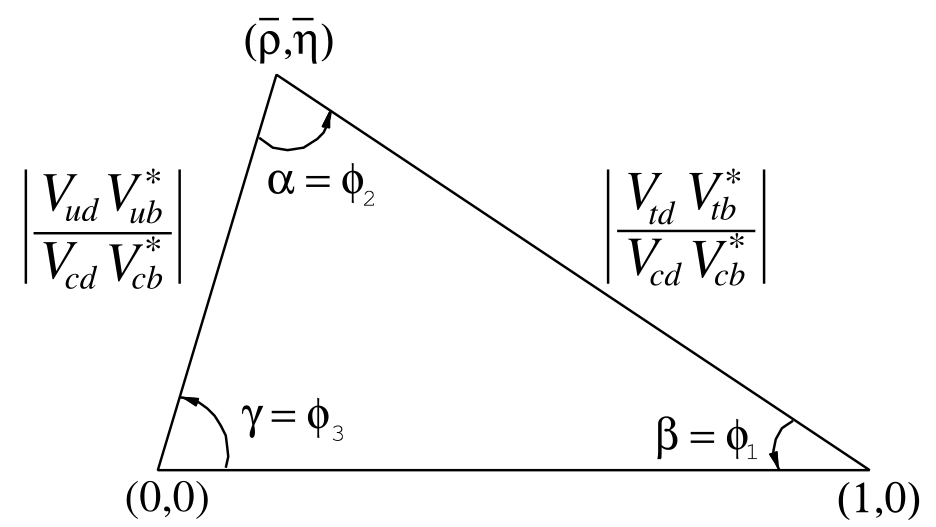
\includegraphics[scale=0.3]{rozdzial1/trojkat.png}
 % Beetle_block.jpeg: 848x489 pixel, 96dpi, 22.44x12.94 cm, bb=0 0 636 367
 \caption{Trójkąt unitarności, kąty $ \phi_{1,2,3}$} są ekwiwalentem do kątów $\alpha,\beta,\gamma$ w notacji używanej przez eksperyment BELLE. Dolny bok trójkąta posiada jednostkową długość jest to zgodne z przyjętą konwencją. 
 \label{fig:trojkat db}
\end{figure}
 

Z eksperymentalnego punktu widzenia, najciekawszym trójkątem jest (db), ponieważ jego boki są porównywalnych rozmiarów co oznacza, że kąty (bądź odpowiadające im fazy) są duże. Rysunek \ref{fig:trojkat db} przedstawia ten trójkąt. Użyto standardowego oznaczenia kątów ($\alpha , \beta , \gamma $), te trzy kąty odnoszą się do zespolonych komponentów macierzy CKM przez związki:

\begin{eqnarray}
\alpha &=& \arg \left(- \frac{V_{td}V^*_{tb}}{ V_{ud}V_{ub}^* }  \right) =\arg \left( \frac{(1-\frac{1}{2} \lambda^2)(i \eta -\rho )}{1-\rho -i\eta}  \right)\\
\beta &=& \arg \left(- \frac{V_{cd}V^*_{cb}}{ V_{td}V_{tb}^* }  \right) =\arg \left( \frac{1}{1-\rho -i\eta}  \right)\\
\gamma &=& \arg \left(- \frac{V_{ud}V^*_{cb}}{ V_{cd}V_{cb}^* }  \right) =\arg \left( 1-\frac{1}{2} \lambda^2 \right) \left( \rho -i \eta \right)
\end{eqnarray} 

Wiele różnych rozpadów mezonów B oraz D można użyć do ograniczania przedziału dostępności dla kątów. Rysunek przedstawia 
 


 \begin{figure}[ht]
 \centering
 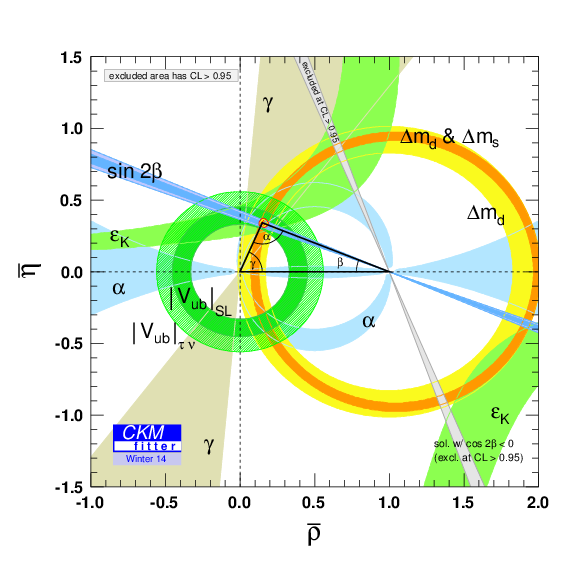
\includegraphics[scale=0.7]{rozdzial1/triangle.png}
 % Beetle_block.jpeg: 848x489 pixel, 96dpi, 22.44x12.94 cm, bb=0 0 636 367
 \caption{Trójkąt unitarności, kąty $ \phi_{1,2,3}$} są ekwiwalentem do kątów $\alpha,\beta,\gamma$ w notacji używanej przez eksperyment BELLE. Dolny bok trójkąta posiada jednostkową długość jest to zgodne z przyjętą konwencją. 
 \label{fig:trojkat wyniki}
\end{figure}



Kusi mnie dodanie podrozdziału o typach łamania symetrii i mieszaniu ogólnie.